\documentclass[12pt, a4paper]{article}
\usepackage[UTF8]{ctex}
\usepackage{amsmath}
\usepackage{amssymb}
\usepackage{amsthm}
\usepackage{geometry}
\usepackage{enumitem}
\usepackage{indentfirst}
\usepackage{caption}
\usepackage{fancyhdr}
\usepackage{booktabs}
\usepackage{titlesec}
\usepackage{draftwatermark}
\usepackage{graphicx} % 导入图像的宏包、单图





% 页面布局设置
\geometry{top=2.54cm, bottom=2.54cm, left=3.18cm, right=3.18cm}

% 行距设置
\linespread{1.5}

%设置水印
\SetWatermarkText{B站：布加拉提}
\SetWatermarkScale{0.4}
% 段落设置
\setlength{\parindent}{2em}
\setlength{\parskip}{0.5em}

% 节标题格式设置
\titleformat{\section}{\normalfont\Large\bfseries}{第\chinese{section}章、}{1em}{}
\titlespacing{\section}{0pt}{2.5ex plus 1ex minus .2ex}{1.3ex plus .2ex}

% 定理环境设置
\newtheoremstyle{solution}
{}
{}
{}
{}
{\bfseries}
{、}
{1em}
{}
\theoremstyle{solution}
\newtheorem{sol}{解}

% 页眉页脚设置
\pagestyle{fancy}
\fancyhf{}
\fancyhead[C]{b站布加拉提整理（回忆版）b站甘茶w独家讲解}
\fancyfoot[C]{\thepage}

\rfoot{整理人：八方\\资源提供：考研乔瑟夫}
\lhead{
\includegraphics[width=0.06\linewidth]{p1.png}}
\rhead{
\includegraphics[width=0.06\linewidth]{p2.png}}
\renewcommand{\headrulewidth}{0.4pt}
\renewcommand{\footrulewidth}{0.4pt}

\begin{document}

\begin{center}
\Large\textbf{2006哈工大硕士考试试题：805物理光学}
\end{center}




\section*{一、解释下列名词（40分）}
\begin{enumerate}
    \item 半波损失
    \item 惠更斯-菲涅尔原理
    \item 倏逝波
    \item 折射定律
    \item 光栅
    \item 法拉第效应
    \item 双折射
    \item 布儒斯特角
    \item 1/4波片
    \item 条纹对比度
\end{enumerate}
\section*{二、简答题（50分）}
\begin{enumerate}
    \item 根据波动理论，简述平面波与球面波的差异
    \item 简述利用单个光源获得相干光的方法，并列干涉装置
    \item (重复)什么是瑞利判据？以望远系统为例说明它对实际光学系统有何意义？
    \item 简述光波干涉与衍射的关系，并举例说明。
    \item 比较棱镜和光栅的色分辨本领的差异。
\end{enumerate}
\section*{三、应用与计算题（40分）}
\begin{enumerate}
    \item 在真空中传播的一列平面电磁波。其电场可表示为\\$E_x=(20V/M)COS[\pi ×10^{14}s^{-1}(t-x/c)+\pi /3],E_y=0,E_z=0$\\问该电磁波的频率，波长，振幅，周期和初相位是多少？
    \item 讨论夫琅和费衍射装置有如下变动时，衍射图样的变化
    \begin{figure}[!htb]
        \centering
        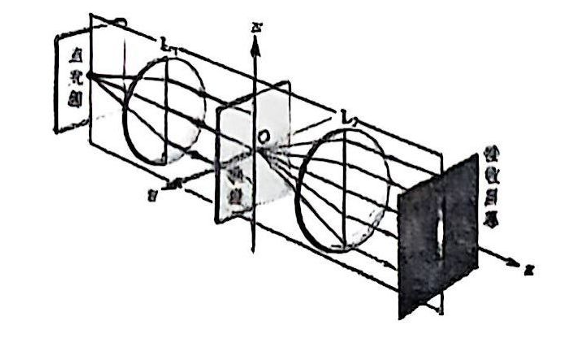
\includegraphics[width=0.7\linewidth]{06.png}
        \caption{我也看不清}
    \end{figure}
    \begin{enumerate}
        \item 增大透镜$L_2$的焦距
        \item 增大透镜$L_2$的口径
        \item 将衍射屏沿光轴z方向前后平移
        \item 衍射屏做垂直于光轴方向移动
        \item 衍射屏绕光轴z旋转
     \end{enumerate}
     在以上哪些情形里零级衍射斑的中心发生移动。
     \item 以纳光观察迈克尔逊干涉条纹，先看到干涉场中12个亮环，且中心是亮点，然后移动一侧反射镜，看到中心消失了10个亮环，此时干涉场中还存在5个亮环。求：
    \begin{enumerate}
        \item 镜面移动的距离
        \item 开始时中心亮斑的级次$k_0$,相对应的等效空气薄膜厚$h_0$
    \end{enumerate}
    \item 一束自然光正入射到重叠的两个偏振片上，如果透射光强为（1）入射光强的1/4（2）透射最大光强的1/4，试确定两个偏振片的夹角。
\end{enumerate}
\section*{四、综合题（20分）}
\begin{enumerate}
    \item 画出迈克尔逊干涉仪原理图
    \begin{enumerate}
        \item 简述其工作原理
        \item 说明它可能有什么用途
        \item 根据你的理解，讨论其时间相干性
        \item 当光源分别为点光源和拓展光源时，讨论干涉条纹的定义域
    \end{enumerate}
\end{enumerate}
\end{document}